\subsection{Discuss the Zeeman Effect in the presence of hyperfine structure.}


\paragraph{Zeemaneffekten:} Idet atomer opfører sig som magnetiske dipoler, da vil man observere et energiskift, hvis atomet indsættes i et eksternt magnetisk felt. Energiskiftet grundet vekselvirkningen mellem atomets dipolmoment og det eksterne magnetfelt vil løfte udartetheden (eng. the degeneracy) af tilstanden, idet man hyperfinstrukturen får en opsplitning i $M_F$.


\paragraph{Hyperfinstruktur:} Hyperfinstrukturen opstår, da man tager højde for kernens impulsmoment. Man bliver nødt til at skifte til at arbejde med det totale atomarimpulsmoment $\Vec{F} = \Vec{I} + \Vec{J}$, hvorved der skiftes basis fra $\ket{I,\: J,\: m_I,\: m_J}$ til $\ket{I,\: J,\: F,\: m_F}$. Energiskiftet grundet finstrukturen findes til at være
\begin{align}
    E_{HFS} &= \frac{A}{2}\left\{F(F+1) - I(I+1) - J(J+1)\right\} \: , \quad \text{med} \quad A = \frac{g_N \mu_N B_J}{\sqrt{J(J+1)}} \: ,
\end{align}
hvor $A$ er \textsf{finstrukturkonstanten} og det resterende kaldes \textsf{intervalfaktoren}.


\paragraph{Zeemaneffekten i hyperfinstruktur:} Som for Zeemaneffekten i finstruktur er der tre tilfælde: Hyperfinstrukturen regnes i et svagt magnetisk felt, et stærkt magnetisk felt, eller et felt med styrke midt i mellem.

\paragraph{Svagt magnetfelt:} I det svage magnetiske felt vil energiskiftet grundet Zeemaneffekten være mindre end energiskiftet grundet hyperfinstrukturen, $E_{ZE}~<~E_{HFS}$, hvorfor Zeemaneffekten kan ses som en perturbation til hyperfinstrukturen, så Hamiltonoperatoren bliver
\begin{align} \label{eq:Q17_StartudtrykForHamiltonForZeemaneffektenSvagtB}
    H_{ZE} &= - \braket{\Vec{\mu}_F} \cdot \Vec{B} \: ,
\end{align}
hvor $\braket{\Vec{\mu}_F}$ er projektionen af $\Vec{\mu}_F$ ind langs $\Vec{F}$, hvilken skal benyttes, da denne er en middelværdi af $\Vec{\mu}_F$ ($\Vec{\mu}_F$ præciserer omkring $\braket{\Vec{\mu}_F}$), og $\braket{\Vec{\mu}_F}$ er velbeskrevet i basen $\ket{I \: J \: F \: M_F}$, hvilket $\Vec{\mu}_F$ ikke er. Denne basis benyttes idet, at vi arbejder med hyperfinstruktur for svage magnetfelter, hvorfor $\Vec{I}$ og $\Vec{J}$ kobler.

Det totale magnetiske dipolmoment for et atom er givet som summen af dipolmomentet grundet elektronens spin og baneimpulsmoment og grundet kerneimpulsmomentet
\begin{align}
    \Vec{\mu}_F &= \Vec{\mu}_I + \Vec{\mu}_J = g_I \frac{\mu_N}{\hbar} \Vec{I} - g_J \frac{\mu_B}{\hbar} \Vec{J} \: ,
\end{align}
hvor $g_N$ er , $\mu_B = e\hbar/(2m_e)$ er Bohrmagnetronen, $g_I$ og $g_J$ er Landé g-faktorer for hhv. kerneimpulsmomentet og elektronimpulsmomentet (samling af baneimpulsmomentet og spinet for elektronen). Derved blive det tidsgennemsnitlige atomerdipolmoment
\begin{align}
    \braket{\Vec{\mu}_F} &= \frac{1}{\abs{\Vec{F}}^2}\left(\Vec{\mu}_F \cdot \Vec{F} \right) \Vec{F}
    = \frac{1}{\abs{\Vec{F}}^2} \left(g_I \frac{\mu_N}{\hbar} \Vec{I} \cdot \Vec{F} - g_J \frac{\mu_B}{\hbar} \Vec{J} \cdot \Vec{F}\right) \Vec{F} \: .
\end{align}

Hamiltonoperatoren fra \cref{eq:Q17_StartudtrykForHamiltonForZeemaneffektenSvagtB} bliver derved, idet $\Vec{B} = B\Hat{z}$,
\begin{align}
    H_{ZE} &= -\left\{\frac{1}{\abs{\Vec{F}}^2} \left(g_I \frac{\mu_N}{\hbar} \Vec{I} \cdot \Vec{F} - g_J \frac{\mu_B}{\hbar} \Vec{J} \cdot \Vec{F}\right) \Vec{F}\right\} \cdot \Vec{B} \nonumber\\
    &= - \frac{1}{\abs{\Vec{F}}^2} \left(g_I \frac{\mu_N}{\hbar} \Vec{I} \cdot \Vec{F} - g_J \frac{\mu_B}{\hbar} \Vec{J} \cdot \Vec{F}\right) B F_z \: ,
\end{align}
hvormed energiskiftet grundet Zeemaneffekten bliver
\begin{align} \label{eq:Q17_StartudtrykForEnergiZeemaneffetenSvagtB}
    E_{ZE,weak\,B} &= \braket{H_{ZE}} = - \frac{1}{\braket{\abs{\Vec{F}}^2}} \left(g_I \frac{\mu_N}{\hbar} \braket{\Vec{I} \cdot \Vec{F} \:} - g_J \frac{\mu_B}{\hbar} \braket{\Vec{J} \cdot \Vec{F} \:}\right) B \braket{F_z} \: .
\end{align}

Forventningsværdien af $\braket{\Vec{I} \cdot \Vec{F}}$ og $\braket{\Vec{J} \cdot \Vec{F}}$ findes ved at $\Vec{F} = \Vec{I} + \Vec{J}$, så
\begin{align}
    \Vec{J} &= \Vec{F} - \Vec{I} \Rightarrow \Vec{J}^2 = \Vec{F}^2 + \Vec{I}^2 - 2\Vec{I} \cdot \Vec{F} \nonumber\\
    \Rightarrow \braket{\Vec{I} \cdot \Vec{F}} &= \frac{1}{2} \left(\braket{\Vec{F}^2} + \braket{\Vec{I}^2} - \braket{\Vec{J}^2}\right) = \frac{\hbar^2}{2} \left\{F(F+1) + I(I+1) - J(J+1)\right\} \: , \\
    \Vec{I} &= \Vec{F} - \Vec{J} \Rightarrow \Vec{I}^2 = \Vec{F}^2 + \Vec{J}^2 - 2\Vec{J} \cdot \Vec{F} \nonumber\\
    \Rightarrow \braket{\Vec{J} \cdot \Vec{F}} &= \frac{1}{2} \left(\braket{\Vec{F}^2} + \braket{\Vec{J}^2} - \braket{\Vec{I}^2}\right) = \frac{\hbar^2}{2} \left\{F(F+1) + J(J+1) - I(I+1)\right\} \: ,
\end{align}
hvorved vi får \cref{eq:Q17_StartudtrykForEnergiZeemaneffetenSvagtB} til at blive
\begin{align} \label{eq:Q17_EnergiZeemanSvagtBfelt}
    E_{ZE,weak\,B} &= - \frac{1}{\hbar^2 F(F+1)} \frac{\hbar^2}{2}\bigg(g_I \frac{\mu_N}{\hbar} \left\{F(F+1) + I(I+1) - J(J+1)\right\} \nonumber\\
    &\qquad \qquad \qquad \qquad \quad - g_J \frac{\mu_B}{\hbar} \left\{F(F+1) + J(J+1) - I(I+1)\right\}\bigg) B \hbar M_F \nonumber\\
    &= - M_F \mu_B B \bigg(g_I \frac{\mu_N}{\mu_B} \frac{F(F+1) + I(I+1) - J(J+1)}{2F(F+1)} \nonumber\\
    &\qquad \qquad \qquad - g_J \frac{F(F+1) + J(J+1) - I(I+1)}{2F(F+1)}\bigg) \nonumber\\
    &= g_F M_F \mu_B B \: ,
\end{align}
hvor Landé g-faktoren for atomarimpulsmomentet er
\begin{align} \label{eq:Q17_gF}
    g_F \equiv g_J \frac{F(F+1) + J(J+1) - I(I+1)}{2F(F+1)} - g_I \frac{\mu_N}{\mu_B} \frac{F(F+1) + I(I+1) - J(J+1)}{2F(F+1)} \: .
\end{align}
Dette kaldes den \textsf{lineære Zeemaneffekt}.\\

Kigger vi på Rubidium-87, der har termsymbolet $5^2S_{1/2}$ og kernekvantetal $I = 3/2$, så får løfter Zeemaneffektetn udartetheden (eng. degeneracy) i $F$, som det kan ses af \cref{fig:Q17_RubidiumHyperFineZeemanSplittings}.
\begin{figure}[!h]
    \centering
    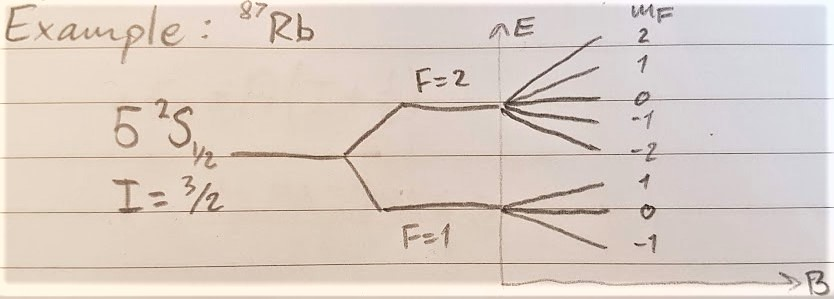
\includegraphics[width=.9\textwidth]{Q17/images/ZeemanEffectWithHyperFineStructureSplittingRubidium.jpg}
    \caption{Opsplitning af Rubidium-87 grundet Zeemaneffekten i et svagt magnetfelt.}
    \label{fig:Q17_RubidiumHyperFineZeemanSplittings}
\end{figure}


\paragraph{Stærkt magnetfelt:} I det stærke magnetfelt, $E_{ZE} > E_{HFS}$, er der tre effekter, som man kigger på
\begin{enumerate}[label=\alph*)]
    \item $\Vec{J}$ præcesserer omkring det eksterne magnetfelt.
    \item $\Vec{I}$ præcesserer omkring det eksterne magnetfelt.
    \item $\Vec{I}$ præcesserer omkring $\Vec{J}$.
\end{enumerate}

\noindent\underline{Effekt a:} Dette er Zeemaneffekten for $\Vec{J}$, hvorfor vi ved, at
\begin{align} \label{eq:Q17_EnergyFromEffectA}
    E_{\text{effect}\,a} &= g_J M_J \mu_B B \: .
\end{align}

\noindent\underline{Effekt b:} Denne effekt er meget lille og bliver derfor negligeret.

\noindent\underline{Effekt c:} Her skal hyperfinstrukturperturbationen laves igen idet, at $\Vec{I}$ og $\Vec{J}$ ikke længere indretter sig efter hinanden\footnote{Dette kaldes Pashen-Backeffekten (eng. the Pashen-Back effect): Impulsmomenterne kobler ikke længere sammen, da deres kobling til det magnetiske felt bliver stærkere end koblingen mellem de to impulsmomenter, så de nu hver især præciserer omkring det magnetiske felt i stedet for, at deres sum præciser rundt om det magnetiske felt.}.
\begin{align}
    H_{HFS,strong\,B} &= - \Vec{\mu}_I \cdot \Vec{B}_J \: ,
\end{align}
så energien bliver
\begin{align} \label{eq:Q17_EnergiStartStaerkBfelt}
    E_{HFS,strong\,B} &= \braket{H_{HFS_strong\,B}} = \braket{- \left(g_I \frac{\mu_N}{\hbar}\Vec{I}\right) \cdot \left(- B_J\frac{\Vec{J} \:}{\abs{\Vec{J}}^2}\right)} \nonumber\\
    &= g_I \frac{\mu_N}{\hbar}B_J \braket{\frac{\Vec{I} \cdot \Vec{J} \:}{\abs{\Vec{J}}^2}} \: .
\end{align}
Der er altså stadig en $\Vec{I} \cdot \Vec{J}$ interaktion, som i hyperfinstrukturen, men $\Vec{I}$ og $\Vec{J}$ orienterer sig efter det eksterne felt og ikke efter hinanden. Derved får vi ???, når $\Vec{B} = B \hat{z}$
\begin{align}
    \overline{\Vec{I} \cdot \Vec{J}} &= \left(\Vec{I}\frac{\Vec{B}}{\abs{\Vec{B}}}\right)\left(\Vec{J}\frac{\Vec{B}}{\abs{\Vec{B}}}\right) = \left(\Vec{I} \cdot \hat{z}\right)\left(\Vec{J} \cdot \hat{z}\right) = I_z J_z \\
    \Rightarrow \braket{\overline{\Vec{I} \cdot \Vec{J}}} &= \braket{I_z J_z} = M_I M_J \hbar \: ,
\end{align}
så energien i \cref{eq:Q17_EnergiStartStaerkBfelt} bliver
\begin{align} \label{eq:Q17_EnergyFromEffectC}
    E_{\text{effect}\,c} &= g_I \frac{\mu_N}{\hbar}B_J \frac{\hbar M_I M_J}{\hbar \sqrt{J(J+1)}} = \frac{g_I \mu_N B_J}{\sqrt{J(J+1)}} M_I M_J = A M_I M_J \: ,
\end{align}
hvor $A$ er finstrukturkonstanten.

\noindent\underline{Sammelagt:} Tilsammen bliver Zeemaneffekten for hyperfinstrukturen i stærke magnetfelter
\begin{align} \label{eq:EnergiskiftZeemanIHyperfinstrukturStarktFelt}
    E_{ZE,strong\,B} &= g_J M_J \mu_B B + A M_I M_J \: .
\end{align}
Dette kaldes den \textsf{ikke-lineære Zeemaneffekt} (eng. non-linear Zeeman effect).


\paragraph{Mellemstærkt magnetisk felt:} I mellemstræke magnetfelter er det lettere besværligt, da man skal ud i at regne udartet perturbationsteori. Der er dog et specialtilfælde for $F = I \pm I$, hvilket ses i alkalimetaller. Her kan man i stedet benytte Breit-Rabi formlen til at bestemme energiskiftet af Zeemaneffekten i hyperfinstrukturen
\begin{align}
    E_{ZE,intermediate\,B} &= - \frac{A}{4} + g_I M_F \mu_N B \pm \frac{\Delta E_0}{2} \left(1 + \frac{4M_F}{2I+1} x + x^2\right) \: ,
\end{align}
hvor
\begin{align}
    \Delta E_0 &= A\left(I + \frac{1}{2}\right) \: , \quad \text{og} \\
    x &= \frac{g_J \mu_B - g_I \mu_N}{\Delta E_0} B \: .
\end{align}



\paragraph{Zeemaneffekt i hyperfinstruktur -- Eksempel hydrogens grundtilstand:} Som eksempel kan vi kigge på finstrukturopsplitningen af hydrogens grundtilstand, hvor $I = J = 1/2$ og $g_J = g_s \simeq 2$.

I det svage magnetfelt får vi for $F = 1$, at $g_F = 1$, så denne vil nu splitte i tre energiniveauer med $M_F = -1,\: 0,\: 1$, som vil være spredt med energien $\mu_B B$ mellem dem. For $F = 0$ bliver $M_F = 0$, så der er opstår ikke en førsteordens Zeemanopsplitning. Dette kan ses af \cref{fig:Q17_AllCasesOfZeemanEffectInHyperFineStructure}.

I det stærke magnetfelt vil de to energiniveauer med $M_J = \pm 1/2$ blive opsplittet til hver to energiniveauer med $M_I = \pm 1/2$, grundet hyperfinstrukturinteraktionen. Disse energiniveauer vil være spredt med energien $A/2$ (uafhængig af magnetfeltets styrke), per \cref{eq:EnergiskiftZeemanIHyperfinstrukturStarktFelt}. Dette kan ses af \cref{fig:Q17_AllCasesOfZeemanEffectInHyperFineStructure}.

Beregning i det mellemstærke magnetfelt overlades til læseren.

\begin{figure}[!h]
    \centering
    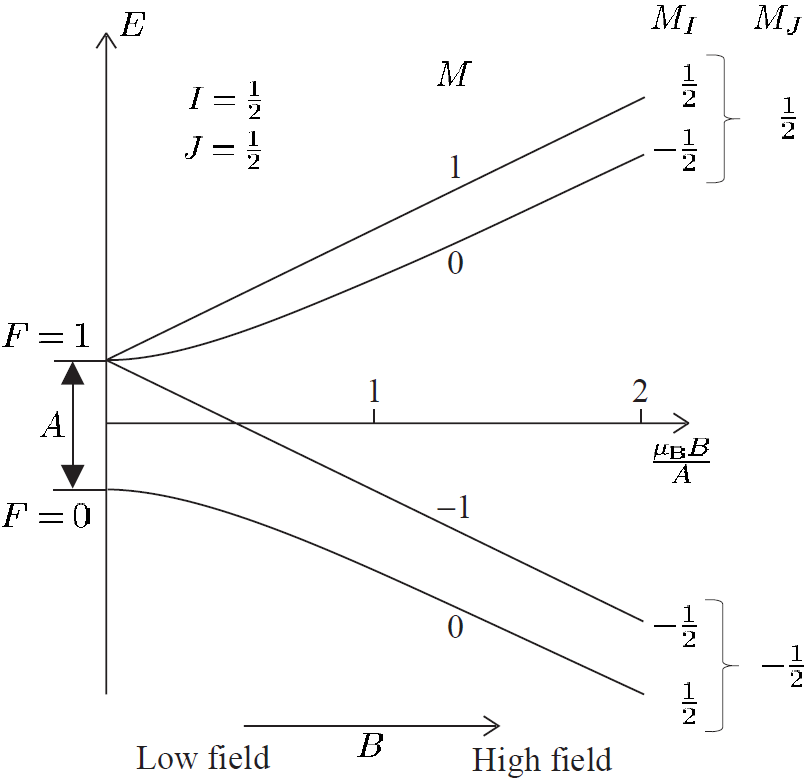
\includegraphics[width=.7\textwidth]{Q17/images/ZeemanEffectHyperFineStructurHydrogenAllCases.PNG}
    \caption{Zeemaneffektens påvirkning af hyperfinstrukturen af grundtilstanden af hydrogen ($1s\:^2 S_{1/2}$). Intervallet mellem $F=0$ og $F=1$ niveauerne  er $A$. Den horisontale akses placering midt mellem energiniveauerne skyldes, at dette hjælper på udregningerne, hvis man går i dybden med udartet perturbationsteori for det mellemstærke magnetfelt. (De to tilstande med $M_F = 0$ er i det svage magnetfelt blandet grundet perturbationen, men flytter sig fra hinanden som det magnetiske felt øges.) Værdien $x = \mu_B B/A$ er afbilledet på den horizontale akse, og svagt felt (low field) og stært felt (high field) regimerne er svarende til hhv. $x \ll 1$ og $x \gg 1$.}
    \label{fig:Q17_AllCasesOfZeemanEffectInHyperFineStructure}
\end{figure}